\chapter{ЭКОЛОГИЯ И ПРОМЫШЛЕННАЯ \\БЕЗОПАСНОСТЬ}
\label{cha:ch_4}

Строгое соблюдение правил безопасности и охраны труда – одно из основных условий работы. Соблюдение заранее оговоренных правил и понимание опасностей при выполнении поставленной задачи, являются главными способами борьбы с травмами и несчастными случаями на производстве. При работе с оборудованием машиностроительного производства и/или опасными веществами риск, которому подвержен работник в случае нарушения правил безопасности значительно выше, чем риск офисного работника.

В данной работе проведен анализ опасных и вредных факторов, влияющих на рабочего, при исполнении технического процесса изготовления переднего днища реактивного двигателя на твёрдом топливе (РДТТ). Процесс будет производится в цехе, в котором установлены различные виды станков. Материал заготовки – сплав СП33.

\section{Анализ опасных и вредных факторов \\ при изготовлении днища двигателя}
Технический процесс изготовления днища РДТТ включает операции и соответствующие им негативные факторы, приведенные в таблице \ref{tab:all_bad_factors}.

\begin{table}[!h]
	\begin{center}
		\caption{Опасные и вредные факторы, возникающие при изготовлении днища двигательной установки}
		\begin{tabular}{|l|p{110mm}|}
  		\hline
Тип операции & Вредные факторы \\ \hline 
Термообработка & Освещение, травмоопасность, вибрации, микроклимат. \\ \hline 
Сверление & Освещение, шум, травмоопасность. \\ \hline 
Фрезерование & Освещение, шум, вредные вещества в воздухе рабочей зоны, вибрации, ЭМИ-поля. \\ \hline 
Растачивание & Освещение, шум, вредные вещества в воздухе рабочей зоны, вибрации. \\ \hline 
Токарная & Освещение, шум, травмоопасность. \\ \hline 
		\end{tabular}
		\label{tab:all_bad_factors}
	\end{center}
\end{table}

Рассмотрев приведенные в таблице факторы, можно заключить, что на рабочего воздействует множество неблагоприятных факторов, способных привести к повышенной утомляемости и, как следствию, травме.

Также на производстве присутствует риск возникновения различных опасных факторов. Согласно ГОСТ 12.0.002-2014, опасным фактором принимается фактор производственной среды и/или трудового процесса, воздействие которого в определенных условиях на организм работающего может привести к травме, в том числе смертельной.

Список опасных факторов, которые возникают при производстве, приведен ниже.

\subsection{Электроопасность}
Основным нормативным документом, связанным с электробезопасностью, являются МПОТ (ПБ) ЭЭУ – Международные правила по охране труда и ГОСТ Р 12.1.019-2009, при эксплуатации электроустановок.
Согласно документу, следует придерживаться следующих правил обеспечения электробезопасности:
\begin{itemize}
	\item Следить за проведением рабочим, причастным к работе с электрооборудованием, инструктажей и обучений безопасным методам и приемам выполнения работ на электроустановках.
	\item Работники должны проходить обучение по оказанию первой помощи пострадавшему на производстве до допуска к самостоятельной работе;
	\item Перед началом работ на электроустановках, следует проверить исправность оборудования, а также следить за состоянием и сообщать специальному персоналу о любых неисправностях оборудования;
	\item Не допускать самовольного проведения работ в действующих электроустановках, а также снабжать персонал необходимым инвентарём для защит от электрического воздействия. 
\end{itemize}

\subsection{Пожарная опасность}
Основные требование, предъявляемые к пожарной безопасности содержатся в нормативном документе СП 4.13130.2013 «Системы противопожарной защиты. Ограничение распространения пожара на объектах защиты. Требования к объемно-планировочным и конструктивным решениям».

Согласно представленному документу, основой средств обеспечения пожарной безопасности является определение класса функциональной пожарной опасности объекта защиты, которая исходит из его целевого назначения и характеристик его основного функционального контингента. Также выбор средств зависит от степени огнестойкости здания.

Основные положения для обеспечения пожарной безопасности при изготовлении днища двигательной установки:
\begin{itemize}
	\item Снабжение производственного цеха переносными огнетушителями (ГОСТ Р 51057-2001);
	\item При работе с горючими, взрывоопасными или легковоспламенимыми веществами, следить за отсутствием по близости источников открытого огня, сварных работ, источников образования искр и т.д;
	\item Помещение должно быть снабжено системами пожаротушения, а работающий в нем персонал должен пройти инструктаж пожарной эвакуации и знать расположение ближайших аварийных выходов и путей следования к ним;
	\item соблюдение порядка хранения веществ и материалов, имеющих опасность воспламенения и тушение которых недопустимо одними и теми же средстваи, в зависимости от их химико-физических свойств.
\end{itemize}

\clearpage
\subsection{Травмоопасность}
Способность опасных производственных факторов при определен-ных обстоятельствах причинить травму работающему. Основным источником травмоопасности на предприятии и при работе в цеху обычно выступают: подвижные части механизмов, машин и узлов; подвижные элементы станков без защиты или экранов; Заготовки, необработанные поверхности, заусенцы, кромки, вылетающая при обработке стружка; падение предметов с высоты.

Основным нормативным документом, описывающим требования к безопасности персонала при работе в цеху, выступает ГОСТ 12.4.125 – 83 Система стандартов безопасности труда (ССБТ). Средства коллективной защиты работающих от воздействия механических факторов. 

\clearpage
Помимо опасных факторов, оператор также подвержен влиянию сле-дующих вредных факторов (фактор производственной среды и/или трудо-вого процесса, воздействие которого в определенных условиях на орга-низм работающего может сразу или впоследствии привести к заболеванию, в том числе смертельному, или отразиться на здоровье потомства постра-давшего, или в отдельных специфичных случаях перехода в опасный про-изводственный фактор - вызвать травму. В безопасности труда применяет-ся концепция порогового воздействия, согласно которой вредный произ-водственный фактор (исключая ионизирующие излучения) неблагоприятно воздействует на организм человека только при превышении интенсивности своего воздействия (и/или полученной дозы) выше некоторого порогового предельно допустимого значения. Последствия этого воздействия могут проявиться сразу (острое заболевание) или спустя какое-то (иногда дли-тельное - годы) время (хроническое заболевание)).

\subsection{Микроклимат}
Под микроклиматом производственных помещений понимаются ме-теорологические условия внутренней среды помещений, которые опреде-ляются действующими на организм человека сочетаниями температуры, влажности, скорости движения воздуха и теплового излучения (СанПин 2.2.4.3359-16). Микроклимат производственных помещений – это ком-плекс физических факторов, оказывающих влияние на теплообмен челове-ка и определяющих самочувствие, работоспособность, здоровье и произ-водительность труда. Поддержание микроклимата рабочего места в пре-делах гигиенических норм – важнейшая задача охраны труда.

Показатели микроклимата:
\begin{itemize}
	\item Температура воздуха;
	\item Относительная влажность воздуха;
	\item Скорость движения воздуха;
	\item Мощность теплового излучения.
\end{itemize}

Воздушная среда из всех элементов, составляющих среду обитания и деятельности человека, является важнейшей. Природный воздух представ-ляет собой сложную динамическую систему, образованную различными газами (и парами) и находящимися во взвешенном состоянии мельчайши-ми твердыми и жидкими частицами – аэрозолями.

Под загрязнением воздуха понимается прямое или косвенное введе-ние в него любого вещества в таком количестве, которое изменяет качество и состав чистого атмосферного воздуха, нанося вред людям, живой и не-живой природе.

Важнейшим газообразным веществом, определяющим качество воздуха, является водяной пар. Чем сильнее нагрет воздух, тем большее количество водяного пара он может содержать. Отношение содержащегося водяного пара к тому предельному количеству, которое может содержаться в воздухе при данной температуре, называется относительной влажностью.

Важнейшей характеристикой воздушной среды является барометрическое давление, поскольку разница барометрического давления и давления воздуха в альвеолах легких определяет величину газообмена. Барометрическое давление считается и называется нормальным на уровне моря (одна атмосфера) и экспоненциально убывает с высотой.

Помимо газового состава и барометрического давления, важнейшей характеристикой воздушной среды служит температура воздуха. В сочетании с подвижностью (скоростью) движения воздуха относительно тела человека температура воздуха определяет характер теплообмена – нагрев или охлаждение тела человека.

Жизнедеятельность человека может нормально протекать лишь при условии сохранения температурного гомеостаза организма, что достигается за счет системы терморегуляции и деятельности других функциональных систем: сердечнососудистой, выделительной, эндо­кринной и систем, обеспечивающих энергетический, водносолевой и белковый обмен.

Для сохранения постоянной температуры тела организм должен находиться в термостабильном состоянии, которое оценивается по тепловому балансу. Тепловой баланс достигается ко­ординацией процессов теплопродукции и теплоотдачи.

Микроклимат по степени влияния на тепловой баланс человека подразделяется на:
\begin{itemize}
	\item нейтральный;
	\item нагревающий;
	\item охлаждающий.
\end{itemize}

Нейтральный микроклимат – это такое сочетание его составляющих, которое при воздействии на человека в течение рабочей смены обеспечивает тепловой баланс организма, разность между величиной теплопродукции и суммарной теплоотдачей находится в пределах $\pm$ 2 Вт, доля теплоотдачи испарением влаги не превышает 30\%.

Охлаждающий микроклимат – это сочетание параметров, при котором имеет место превышение суммарной теплоотдачи в окружающую среду над величиной теплопродукции организма, приводящее к образованию общего и/или локального дефицита тепла в теле человека (> 2 Вт).

Охлаждающий микроклимат приводит к обострению язвенной болезни, радикулита, обусловливает возникновение заболеваний органов дыхания, сердечно-сосудистой системы. Охлаждение человека (как общее, так и локальное) приводит к изменению его двигательной реакции, нарушает координацию и спо­собность выполнять точные операции, вызывает тормозные процессы в коре головного мозга, что может быть причиной возникновения различ­ных форм травматизма. При локальном охлаждении кистей снижается точность выполнения рабочих операций.

Нагревающий микроклимат – сочетание его параметров, при котором имеет место изменение теплообмена человека с окружающей средой, проявляющееся в накоплении тепла в организме (> 2 Вт) и/или в увеличении доли потерь тепла испарением влаги (>30\%).

Воздействие нагревающего микроклимата вызывает нарушение состояния здоровья, снижение работоспособности и производительности труда. Нагревающий микроклимат может привести к заболеванию общего характера, которое проявляется чаще всего в виде теплового коллапса. Он возникает вследствие расширения сосудов и уменьшения давления в них крови. Обморочному состоянию предшествует головная боль, чувство слабости, головокружение, тошнота.

Тепловой удар очень опасен. Даже при раннем выявлении каждый пятый случай является смертельным. При общем тепловом застое значительно повышается температура тела, что приводит к прямому повреждению тканей, особенно центральной периной системы. Тошнота и рвота предшествуют шоковой стадии с глубокой потерей сознания, иногда сопровождающейся судорогами. Вследствие расстройства центра терморегуляции снижается потообразование. Кожа горячая, сухая, сначала имеет красный цвет, а потом приобретает серую окраску. Смертность тем выше, чем выше температура тела.

В результате солнечного удара в первую очередь нарушаются функции головного мозга из-за местного перегревания незащищенной от солнца головы. 

\begin{table}[!h]
	\begin{center}
		\caption{Параметры нормирования микроклимата, СанПиН 2.2.4.1191-03}
		\begin{tabular}{|p{21mm}|p{27mm}|p{19mm}|p{27mm}|p{33mm}|p{21mm}|}
  		\hline
Период года	& Категория работы по уровням энерготрат, Вт & Темпера- тура, °С & Температура поверхностей, °С	& Относительная влажность, \% &	Скорость движения воздуха, м/с, не более \\ 
	\hline
 Холодный & Iа (до 139) & 22-24 & 21-25  & 40-60 & 0,1 \\ 
  &Iб (140-174) &21-23 &20-24 &  &0,1 \\
  &IIа (175-232) &19-21 &18-22 &  &0,2 \\
  &IIб (233-290) &17-19 &16-20 &  &0,2 \\
  &III (более 290) &16-18 &15-19 &  &0,3 \\ \hline

 Тёплый	 & Iа (до 139) &23-25   &22-26  & 40-60 &0,1  \\ 
  &Iб (140-174) & 22-24&21-25 &  & 0,1 \\ 
  &IIа (175-232) &20-22 &19-23 &   &0,2 \\
  &IIб (233-290) &19-21 &18-22 &   &0,2 \\
  &III (более 290) &18-20 &17-21 &   &0,3 \\ \hline
		\end{tabular}
		\label{tab:eco_climat}
	\end{center}
\end{table}

Тепловое состояние человека – это функциональное состояние организма, обусловленное его теплообменом с окружающей средой, характеризующееся содержанием и распределением тепла в глубоких и поверхностных тканях организма, а также степенью напряжения механизмов терморегуляции.

Теплового состояние человека классифицируется на:
\begin{itemize}
	\item оптимальное;
	\item допустимое;
	\item предельно допустимое;
	\item недопустимое.
\end{itemize}

Разработан метод оценки теплового состояния в целях обоснования гигиенических требований к микроклимату рабочих мест, а также меры профилактики по защите работающих от возможного охлаждения и перегревания.

По степени влияния на самочувствие человека, его работоспособность микроклиматические условия подразделяются на:
\begin{itemize}
	\item оптимальные;
	\item допустимые;
	\item вредные;
	\item опасные.
\end{itemize}

Нормативные гигиенические требования к отдельным показате­лям микроклимата, их сочетаниям, разработанные на основе изучения теплообмена и теплового состояния организма человека в микро­климатических камерах и в производственных условиях, а также на основе клинических и эпидемиологических исследований, изложены в СанПиН 2.2.4.3359-16.

\paragraph{Защита работников от перегревания и переохлаждения}
Профилактика перегрева организма работника в нагревающем микроклимате включает следующие мероприятия:
\begin{itemize}
	\item нормирование верхней границы внешней термической нагрузки на допустимом уровне применительно к восьмичасовой рабочей смене;
	\item регламентация продолжительности воздействия нагревающей среды для поддержания среднесменного теплового состояния на опти­мальном или допустимом уровне;
	\item использование специальных средств коллективной и индивиду­альной защиты, уменьшающих поступление тепла извне к поверхности тела человека и обеспечивающих допустимый тепловой режим.
Защита от охлаждения осуществляется посредством:
	\item одежды, изготовленной в соответствии с требованиями государственных стандартов.
	\item использования локальных источников тепла, обеспечивающие сохранение должного уровня общего и локального теплообмена организма.
	\item регламентации продолжительности непрерывного пребывания на холоде и продолжительности пребывания в помещении с комфортными условиями. 
\end{itemize}

\paragraph{Аэроионный состав воздуха в производственных \\помещениях}

Наряду с температурой, влажностью, скоростью движения воздуха в производственных помещениях на жизнедеятельность человека оказывает влияние аэроионный состав воздуха.

В помещениях с отрицательными ионами происходит уменьшение количества микроорганизмов, снижается концентрация пыли в воздухе, нейтрализуются некоторые газы, устраняются электростатические заряды с поверхностей оборудования.

Ионизация воздуха – процесс превращения нейтральных атомов и молекул воздушной среды в электрически заряженные частицы (ионы).

В воздухе всегда имеются различные включения в виде мельчайших пылинок – аэрозолей, водяных паров и других посторонних примесей. Встречая на пути движения эти взвешенные частицы, легкие ионы соеди-няются с ними, сообщая им свой заряд. В результате таких соединений частиц образуются заряженные частицы, которые получили название тяжелых ионов. Тяжелые положительно заряженные ионы в воздухе помещений могут вызывать на коже человека угревую сыпь, прыщи, снижать эластичность кожи. Существуют сверхтяжелые ионы, которые называют аэрозолями. Они состоят из копоти, тумана, мелких дождевых капель. Такие частицы могут иметь много элементарных электрических зарядов и не нести на себе ни единого истинного газового иона.

Воздух, содержащий отрицательные аэроионы, является своеобразным экраном, отражающим излучения положительных ионов от дисплеев, телевизоров и другой оргтехники.

Естественная ионизация происходит в результате воздействия на воздушную среду космических излучений и частиц, выбрасываемых радиоактивными веществами при их распаде.

Технологическая ионизация происходит при воздействии на воздушную среду радиоактивного, рентгеновского и ультрафиолетового излучений, термоэмиссии, фотоэффекта и других ионизирующих факторов, обусловленных технологическим процессом.

Искусственная ионизация осуществляется специальными устройствами – аэроионизаторами. Физической основой большинства аэроионизаторов является коронный электрический разряд, позволяющий получать ионы нужной полярности и исключать образование вредных химических соединений (озон и окислы азота).

Нормативные уровни ионизации воздуха в производственных и общественных помещениях приведены в санитарных правилах и нормативах СанПиН 2.2.4.1294-03 “Физические факторы производственной среды. Гигиенические требования к аэроионному составу воздуха производственных и общественных помещений”. Согласно этому документу регламентируют: минимально допустимый уровень, максимально допустимый уровень, коэффициент униполярности.

Минимально допустимый и максимально допустимый уровни ионизации воздуха определяют диапазон концентраций аэроионов обеих полярностей и коэффициента униполярности во вдыхаемом воздухе, отклонение от которых создает угрозу здоровью человека. Нормативные значения уровней ионизации воздуха приведены в таблице \ref{tab:eco_ion}.

\clearpage
Измерение числа ионов в порядке текущего надзора производится один раз в квартал, а также в следующих случаях:
\begin{itemize}
	\item при аттестации рабочих мест;
	\item при организации новых рабочих мест;
	\item при внедрении новых технологических процессов, потенциально мо-гущих изменить ионный режим в зоне дыхания персонала;
	\item при оснащении рабочих мест аэроионизаторами.
\end{itemize}

\begin{table}[!h]
	\begin{center}
		\caption{Параметры нормирования микроклимата, СанПиН 2.2.4.1191-03}
		\begin{tabular}{|p{35mm}|p{27mm}|p{19mm}|p{35mm}|}
	\hline
	Нормируемые уровни & \multicolumn{2}{|c|}{Число ионов в 1 $\text{см}^3$ воздуха $\rho$ } & Коэффициент униполярности У \\
	\cline {2-3}
	& $\rho^\text{+}$ & $\rho^\text{-}$ &  \\ \hline
	Минимально допустимый & $\ge 400$ & > 600 &  $0.4 \le \text{У} \le 1.0 $ \\
	\cline {2-3}
	Максимально допустимый& \multicolumn{2}{|c|}{ <50 000 } &  \\ 
	\hline
		\end{tabular}
		\label{tab:eco_ion}
	\end{center}
\end{table}

Для современных офисных помещений задачу нормализации аэроионного состава воздуха целесообразно решать, используя ионизаторы, встраиваемые в приточные воздуховоды вентиляционных систем. Применение приточно-вытяжной вентиляции способно обеспечить относительно равномерное распределение аэронов по помещению и исключить возможность их накопления в локальных зонах. Устанавливать ионизаторы следует на незначительном расстоянии от выходной вентиляционной решетки или системы раздачи воздуха в помещение, что обусловлено значительными «потерями» аэроионов при их движении по воздуховодам (как металлическим, так и диэлектрическим) за счет нейтрализации зарядов при контакте с поверхностями.

\subsection{Вибрации}
Нормативный документ описывающий вибрации возникающие в процессе работы станков и инструментов – СН 2.2.4/2.1.8.566-96 Производственная вибрация, вибрация в помещениях жилых и общественных зданий. Санитарные нормы.

Согласно документу, вибрации классифицируются по способу передачи на человека:
\begin{itemize}
	\item общую вибрацию, передающуюся через опорные поверхности на тело сидящего или стоящего человека; 
	\item локальную вибрацию, передающуюся через руки человека.
По источнику возникновения вибраций различают:	
	\item локальную вибрацию, передающуюся человеку от ручного механизированного инструмента (с двигателями), органов ручного управления машинами и оборудованием;	
локальную вибрацию, передающуюся человеку от ручного немеханизированного инструмента (без двигателей), например, рихтовочных молотков разных моделей и обрабатываемых деталей; 
	\item общую вибрацию 1 категории - транспортную вибрацию, воздействующую на человека на рабочих местах самоходных и прицепных машин, транспортных средств при движении по местности, агрофонам и дорогам (в том числе при их строительстве). К источникам транспортной вибрации относят: тракторы сельскохозяйственные и промышленные, самоходные сельскохозяйственные машины (в том числе комбайны); автомобили грузовые (в том числе тягачи, скреперы, грейдеры, катки и т.д.); снегоочистители, самоходный горно-шахтный рельсовый транспорт;
	\item общую вибрацию 2 категории - транспортно-технологическую вибрацию, воздействующую на человека на рабочих местах машин, перемещающихся по специально подготовленным поверхностям производственных помещений, промышленных площадок, горных выработок. К источникам транспортно-технологической вибрации относят: экскаваторы (в том числе роторные), краны промышленные и строительные, машины для загрузки (завалочные) мартеновских печей в металлургическом производстве; горные комбайны, шахтные погрузочные машины, самоходные бурильные каретки; путевые машины, бетоноукладчики, напольный производственный транспорт;
	\item общую вибрацию 3 категории - технологическую вибрацию, воздействующую на человека на рабочих местах стационарных машин или передающуюся на рабочие места, не имеющие источников вибрации. К источникам технологической вибрации относят: станки металло- и деревообрабатывающие, кузнечно-прессовое оборудование, литейные машины, электрические машины, стационарные электрические установки, насосные агрегаты и вентиляторы, оборудование для бурения скважин, буровые станки, машины для животноводства, очистки и сортировки зерна (в том числе сушилки), оборудование промышленности стройматериалов (кроме бетоноукладчиков), установки химической и нефтехимической промышленности и др.
\end{itemize}

\begin{table}[!h]
	\begin{center}
		\caption{Гигиенические нормы вибрации по СН 2.2.4/2.1.8.556-96}
		\begin{tabular}{|p{30mm}|
			p{7mm}|
			p{7mm}|
			p{7mm}|
			p{7mm}|
			p{7mm}|
			p{7mm}|
			p{7mm}|
			p{7mm}|
			p{7mm}|
			p{7mm}|
			p{10mm}|
		}
	\hline
	Вид вибрации & \multicolumn{11}{|p{110mm}|}{Допустимый уровень виброскорости, дБ, в октавных полосах со среднегеометрическими частотами, Гц} \\ 
	\cline {2-12}
	& 1 & 2 & 4 & 8 & 16 & 31,5 & 63 & 125 & 250 & 500 & 1000 \\
	\hline
	Технологиче- ская & - & 108 & 99 & 93 & 92 & 92 & 92 & - & - & - & - \\
	\hline
		\end{tabular}
		\label{tab:eco_vibro}
	\end{center}
\end{table}

Общую вибрацию категории 3 по месту действия подразделяют на следующие типа:
\begin{itemize}
	\item на постоянных рабочих местах производственных помещений предприятий;
	\item на рабочих местах на складах, в столовых, бытовых, дежурных и других производственных помещений, где нет машин, генерирующих вибрацию;
	\item на рабочих местах в помещениях заводоуправления, конструкторских бюро, лабораторий, учебных пунктов, вычислительных центров, здравпунктов, конторских помещениях, рабочих комнатах и других помещениях для работников умственного труда;
\end{itemize}

Для борьбы с вибрациями, возникающими при работе станков и инструментов, подходящим вариантом будет подготовка фундамента специальной структуры и состава.

\subsection{Шум}
Основными источниками шума на рабочем месте являются:
\begin{itemize}
	\item Работающие станки и инструменты;
	\item Падающие предметы и перемещаемые заготовки;
	\item Фоновый шум со стороны окружающей застройки, транспортных магистралей и т.д.
\end{itemize}

Нормативный документ применимый к урегулированию уровня шума – СанПиН 2.2.4/2.1.8.562-96 «Шум на рабочих местах, в помещениях жилых, общественных зданий и на территории жилой застройки»
\begin{table}[!h]
	\begin{center}
		\caption{Допустимые уровни звукового давления на рабочих местах и в производственных помещениях}
		\begin{tabular}{|p{29mm}|
			p{8mm}|
			p{6mm}|
			p{6mm}|
			p{6mm}|
			p{6mm}|
			p{8mm}|
			p{8mm}|
			p{8mm}|
			p{6mm}|
				p{30mm}|
		}
	\hline
	Рабочие места & \multicolumn{9}{|p{100mm}|}{Уровни звукового давления, дБ, в октавных полосах со среднегеометрическими частотами, Гц } & Уровни звука и эквивалентные уровни звука, дБа \\
	\cline {2-10}
	& 31.5 & 63 & 125 & 250 & 500 & 1000 & 2000 & 4000 & 8000 & \\
	\hline
	В производственных помещениях и на территории предприятий & 107 & 95 & 87 & 82 & 78 & 75 & 73 & 71 & 69 & 80 \\
	\hline
		\end{tabular}
	\end{center}
\end{table}

\clearpage
Согласно таблице \ref{tab:eco_sound_pressure}, в зависимости к соответствующей трудовой деятельности следует рассматривать различные нормы допустимого звукового давления. В рассматриваемом случае данное значение – 65 дБ.
Рекомендациями для увеличения комфортабельности работы и снижению шумовой нагрузке, будут являться:
\begin{itemize}
	\item Своевременная сменный ремонт, смазка и настройка используемого оборудования;
	\item Достижение снижения уровня шума, путем акустической обработки ограждающих поверхностей помещения;
	\item Использование специальных красок и материалов, уменьшающих шум, издаваемый оборудованием.
\end{itemize}

\begin{table}[!h]
	\begin{center}
		\caption{Допустимые уровни звукового давления в зависимости от категории тяжести трудового процесса}
		\begin{tabular}{|p{35mm}|
			p{20mm}|
			p{20mm}|
			p{20mm}|
			p{20mm}|
			p{20mm}|
		}
	\hline
Категории напряженности трудового процесса & \multicolumn{5}{|p{100mm}|}{ Категории тяжести трудового процесса } \\
	\cline {2-6}
	& Легкая физическая нагрузка	 & Средняя физическая нагрузка	 & Тяжелый труд 1 степени & Тяжелый труд 2 степени	& Тяжелый труд 3 степени \\ \hline
Напряженность легкой степени  &  80  &  80  &  75  &  75  &  75 \\ \hline
Напряженность средней степени  &  70  &  70  &  65  &  65  &  65 \\ \hline
Напряженный труд 1 степени  &   60  &  60  &  -  &  -  &  - \\ \hline
Напряженный труд 2 степени  &   50  &  50  &  -  &  -  &  - \\
	\hline
		\end{tabular}
		\label{tab:eco_sound_pressure}
	\end{center}
\end{table}

\subsection{Освещение}
Действующие нормы производственного освещения описываются нормативным документом СНиП 23.05-95* Естественное и искусственное освещение.

Правильно спроектированное помещение, с необходимым количеством осветительных приборов и правильным их расположением, обеспечивают возможность нормальной производственной деятельности. При недостатках освещенности, могут возникнуть проблемы со зрением, повышенная утомляемость, нарушение центральной нервной системы, а также это может привести к травмам или нарушить общую безопасность на производстве.

В свою очередь, оказание необходимого уровня освещения позволяет обеспечить на рабочем месте необходимую производительность труда и качество выпускаемой продукции.

В рассматриваемом случае рассматривается ситуация, когда ведутся работы очень высокой точности. При этом контрастность объекта с фоном средняя, как и характеристика фона. В связи с этим при системе комбинированного освещения значение нормированной минимальной освещенности составляет Еmin=300 лк.

\section{Расчёт искусственного освещения \\рабочего помещения}
Поскольку одним из основных недостатков концентрических ПОУ являются высокие требования к точности изготовления, необходимо создать достаточно благоприятные условия для изготовления оных. Важнейшим фактором в этом случае будет являться освещение цеха, расчёт которого и будет произведён в этом разделе.

Рассчитать систему искусственного освещения для создания на рабочих местах нормируемой освещённости в цехе для механической обработки размерами: длина А =50 м, ширина В = 20 м, высоте Н = 9 м. В цехе выполняются работы высокой точности (наименьшие размеры объектов различения 0,15 мм), фон - темный, контраст - средний, выделение пыли -  значительное. 

Выбираем дуговые ртутные люминесцентные лампы (ДРЛ), рекомендуемые для высоких цехов при работе с поверхностями без выраженной цветности (металл); выбираем общее освещение, так как до всей площади помещения выполняются однотипные работы; для ламп ДРЛ рекомендуются специальные светильники СЗ4ДРЛ прямого свете с зеркальной отражающей поверхностью, так как помещение высокое, а отражающая способность стен и потолка малая. 

Размещаем светильники равномерно четырьмя рядами (рисунок \ref{fig:plant_light_scheme}). Расстояние между рядами светильников L определяем на условия:

$$ \frac{L}{3} + L + L + L + \frac{L}{3} = B \Rightarrow L = \frac{20 \cdot 3}{11}=5.45 м; \frac{L}{3} = 1.81 м $$

\begin{figure}[!h]
\begin{center}
	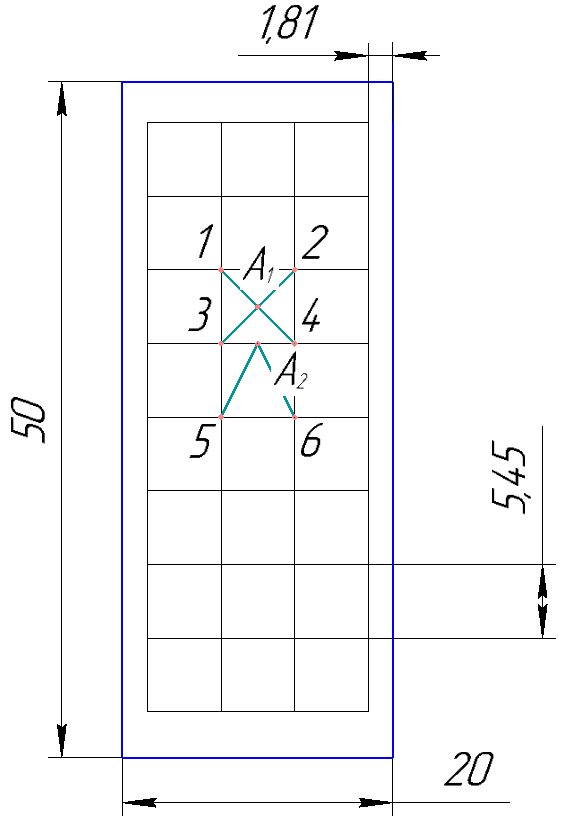
\includegraphics[height=10cm]{plant_light_scheme}
	\caption{Схема размещения светильников}
	\label{fig:plant_light_scheme}
\end{center}
\end{figure}

Количество светильников в ряду:
$$ \frac{A}{L} = \frac{50}{5.45} = 9 $$

Общее число светильников:
$$ N = 4 \cdot 9 = 36 $$

Высоту повеса светильников над уровнем пола определяем из условия их наиболее выгодного светотехнического расположения:
$$ h =L \cdot \lambda=5,45 $$

Значение h оказалось больше минимально допустимой высоты подвеса светильников над полом, следовательно, выполнено требование норм по ограничению ослепленности осветительной установкой. 

В соответствии с характером работ, системой освещения и типом источника света минимальная нормируемая освещённость Е= 300 лк, коэффициент запасе k = 1,8.

Проводим расчет по точечному методу, рекомендуемому для больших цехов с малой долей отражённого света, для контрольных точек А1 и А2 (рисунок \ref{fig:plant_light_scheme}). Ниже приводится порядок этого расчета, а его результаты сведены в таблице \ref{tab:ecolog_results}:
\begin{enumerate}[1.]
	\item Тангенс угла падения светового луча от ближайших светильников tg $\alpha=\frac{d}{h}$, где d - проекция расстоянии от контрольной точки до светильника на горизонтальную плоскость (определяется по чертежу), h - высота подвеса светильника, h= 5,45 м;
	\item Угол $\alpha$ и $\cos \alpha$ определяем по найденному значению $\tg \alpha$;
	\item Силу света $J_\alpha$ условной рампы в 1000 лм для выбранного типа светильника и угла $\alpha$ определяем из методического пособия  \cite{ECO};
	\item Освещенность от i-го светильника в расчетных точках определяем по формуле $E_{Аi}=\frac{J_\alpha \cdot \cos^3 \alpha \cdot \mu}{k \cdot h^3 } $ где $\mu$ - коэффициент, учитывающий действие удаленных светильников ($\mu$= 1,15);
	\item Суммарная освещенность в каждой из контрольных точек, создаваемая ближайшими светильниками: $E_A = \sum_{i=1}^n E_{Ai} $;
	\item Расчётный световой поток (в люменах), который должен быть создан каждой лампой для получения в расчётной точке нормируемой освещённости $E_\text{н}$: F=1000 $\frac{E_H}{E_A}$ ;
	\item Подбираем в соответствии с полученным значением F лампу требуемой мощности $P_A$. При выборе мощности лампы следует принимать значение ближайшего большого светового потока;
	\item Суммарная мощность имеющейся в производственном помещении осветительной установки: $P_\Sigma = P_A \cdot N $=25200 Вт.
\end{enumerate}

\begin{table}[!h]
	\begin{center}
		\caption{Результаты проверки на контрольных точках}
		\begin{tabular}{|p{22mm}|
			p{25mm}|
			p{8mm}|
			p{12mm}|
			p{10mm}|
			p{10mm}|
			p{10mm}|
			p{10mm}|
			p{11mm}|
			p{8mm}|
		}
	\hline
	Контроль- ная точка  & Светильник № & d,м & $\tg \alpha$ & $\alpha$,° & $J_\alpha$, кв & $E_{Ai}$, лк & $E_A$, лк & F, лм & $P_A$, Вт  \\
	\hline
 	A1 & 1 & 3,86 & 0,708 & 35,3&  305 &2,55 & 10,2 & 29412 & 700 \\
	\cline {2-8}
& 2 & 3,86 & 0,708 & 35,3 & 305 & 2,55 & 10,2 & & \\ 
	\cline {2-8}
& 3 & 3,86 & 0,708 & 35,3 & 305 & 2,55 & 10,2 & & \\
	\cline {2-8}
& 4 & 3,86 & 0,708 & 35,3 & 305 & 2,55 & 10,2 & & \\
	\hline
 	A2 & 3 & 2,73 & 0,5 & 27 &  305 & 4,2 & 10,1 & 29703  & 700 \\
	\cline {2-8}
& 4 & 2,73 & 0,5 & 27 & 305 & 4,2 & 10,1 & & \\
	\cline {2-8}
& 1 & 6,1 & 1,12 & 50 & 305 & 0,44 & 10,1 & & \\
	\cline {2-8}
& 2 & 6,1 & 1,12 & 50 & 305 & 0,44 & 10,1 & & \\
	\cline {2-8}
& 5 & 6,1 & 1,12 & 50 & 305 & 0,44 & 10,1 & & \\
	\cline {2-8}
& 6 & 6,1 & 1,12 & 50 & 305 & 0,44 & 10,1 & & \\
	\hline
		\end{tabular}
		\label{tab:ecolog_results}
	\end{center}
\end{table}

\section{Экологическая экспертиза проекта}
\paragraph{Утилизация и переработка металлической стружки}

Высокопроизводительные металлообрабатывающие станки, использующие скоростную резку, нуждаются в больших объемах охлаждающей жидкости и производят огромное количество металлической пыли и стружки. Использование таких станков приводит к интенсивному использованию металла, ресурсы которого неумолимо сокращаются. Это приводит к дефициту и подорожанью этого сырья. Учитывая, что запасы руды небезграничны, а легкодоступный металлический лом практически исчерпан, возникает вопрос поиска новых возможностей пополнения сырья для возобновления запасов металла.

Одним из таких способов является сбор и последующая переработка металлической стружки, которая возникает в процессе обработки различных деталей на металлообрабатывающих станках.

Металлическая стружка является продуктом обработки различных металлических деталей с помощью разного рода технологического оборудования.

В процессе работы с деталями на заводах и предприятиях может образовываться большое количество стружки, общий вес которой может составлять до 10\% от массы обрабатываемых деталей. Это очень большое количество отходов, которые могут успешно применяться в процессе повторной переработки для получения новых металлических заготовок.

Сбор и транспортировка стружки осложняется тем, что эти отходы имеют небольшую плотность. Это приводит к тому, что контейнер для сбора металлической стружки быстро наполняется, а для перевозки отходов на перерабатывающее предприятие требуется большое количество транспортных средств или много дополнительных рейсов.

Проблемы возникают и в процессе переработки необработанной стружки. Если переплавка производится непрессованной стружки, то возникают существенные потери металла вследствие большого угара этого вторсырья и окисления легирующих элементов, содержащихся в стальной стружке. Это в свою очередь приводит к снижению качества получаемой стали.

Чтобы исключить перечисленные проблемы, на предприятиях используют специальные механизированные системы для сбора, хранения и транспортировке стружки и подготовки ее к последующей утилизации и переработке.

Переработка производственных отходов в виде металлической стружки подразумевает под собой повторную переплавку этого вторсырья с целью получения нового металла.


\paragraph{Утилизация стружки чёрных металлов}

Большой процент металлической стружки приходится на черные металлы (сталь, чугун). Прием стружки металлической черных металлов производится в соответствии с ГОСТом 2787-75, который определяет классы стружки и требования к ее состоянию.

К основным особенностям относится то, что стружка не должна иметь ржавчину, за исключением небольшого налета, также не должно быть следов воздействия отжига, кислоты. Ограничено и наличие маслянистых отложений на металлической стружке.

Если стружка соответствует описным в ГОСТе параметрам, она отправляется на повторную переплавку.

\paragraph{Утилизация стружки цветных металлов}

Переработка металлической стружки цветных металлов имеет свои особенности, которые связаны с выполнением определенных условий по чистоте стружки от различных примесей. Отбор и процесс переработки цветной стружки регламентируется ГОСТом 28053-89. В нем описаны рекомендации по выбору и использованию методик для отбора стружки.
На крупных перерабатывающих предприятиях используют несколько методов для распределения стружки по категориям:
\begin{itemize}
	\item визуальный осмотр;
	\item учет магнитных свойств материала;
	\item химический анализ состава.
\end{itemize}
После соответствующего отбора стружка отправляется на переплавку, в процессе которой могут отбираться пробы для проведения спектрального анализа чистоты получаемого металла.

\paragraph{Оборудование для утилизации}

Процесс утилизации металлической стружки упрощается за счет использования специальных механизированных комплексов, которые позволяют подготовить вторсырье для последующей переплавки. Эти комплексы включают в свой состав различное функциональное оборудование.

\paragraph{Дробилки}

Эти установки используются для измельчения металлических отходов с целью того, чтобы на выходе была мелкая металлическая стружка, которая впоследствии будет брикетирована.

Дробилки позволяют измельчать стружку за счет ее резанья, трения друг о друга. Такие установки подходят для дробления как отходов черных материалов, так и цветных.

\paragraph{Центрифуги}

Установки этого типа применяются для очистки и осушения дробленной металлической стружки.

С помощью этих устройств можно выделить из стружки остатки масла и различных эмульсий и произвести сушку металла перед его брикетированием.

\paragraph{Прессы}

Это установки, с помощью которых осуществляется прессование металлической стружки.

После обработки на прессе получают компактные брикеты с высокой плотностью, из которых получают высококачественный переплавленный металл.
